% Template for Cogsci submission with R Markdown

% Stuff changed from original Markdown PLOS Template
\documentclass[10pt, letterpaper]{article}

\usepackage{cogsci}
\usepackage{pslatex}
\usepackage{float}
\usepackage{caption}

% amsmath package, useful for mathematical formulas
\usepackage{amsmath}

% amssymb package, useful for mathematical symbols
\usepackage{amssymb}

% hyperref package, useful for hyperlinks
\usepackage{hyperref}

% graphicx package, useful for including eps and pdf graphics
% include graphics with the command \includegraphics
\usepackage{graphicx}

% Sweave(-like)
\usepackage{fancyvrb}
\DefineVerbatimEnvironment{Sinput}{Verbatim}{fontshape=sl}
\DefineVerbatimEnvironment{Soutput}{Verbatim}{}
\DefineVerbatimEnvironment{Scode}{Verbatim}{fontshape=sl}
\newenvironment{Schunk}{}{}
\DefineVerbatimEnvironment{Code}{Verbatim}{}
\DefineVerbatimEnvironment{CodeInput}{Verbatim}{fontshape=sl}
\DefineVerbatimEnvironment{CodeOutput}{Verbatim}{}
\newenvironment{CodeChunk}{}{}

% cite package, to clean up citations in the main text. Do not remove.
\usepackage{apacite}

% KM added 1/4/18 to allow control of blind submission


\usepackage{color}

% Use doublespacing - comment out for single spacing
%\usepackage{setspace}
%\doublespacing


% % Text layout
% \topmargin 0.0cm
% \oddsidemargin 0.5cm
% \evensidemargin 0.5cm
% \textwidth 16cm
% \textheight 21cm

\title{How to Make a Proceedings Paper Submission}

\usepackage{float} \floatplacement{figure}{T} \usepackage{graphicx}
\usepackage{booktabs}
\usepackage{longtable}
\usepackage{array}
\usepackage{multirow}
\usepackage{wrapfig}
\usepackage{float}
\usepackage{colortbl}
\usepackage{pdflscape}
\usepackage{tabu}
\usepackage{threeparttable}
\usepackage{threeparttablex}
\usepackage[normalem]{ulem}
\usepackage{makecell}
\usepackage{xcolor}

\author{{\large \bf Morton Ann Gernsbacher (MAG@Macc.Wisc.Edu)} \\ Department of Psychology, 1202 W. Johnson Street \\ Madison, WI 53706 USA \AND {\large \bf Sharon J.~Derry (SDJ@Macc.Wisc.Edu)} \\ Department of Educational Psychology, 1025 W. Johnson Street \\ Madison, WI 53706 USA}

\newlength{\cslhangindent}
\setlength{\cslhangindent}{1.5em}
\newenvironment{CSLReferences}%
  {}%
  {\par}

\begin{document}

\maketitle

\begin{abstract}
Include no author information in the initial submission, to facilitate
blind review. The abstract should be one paragraph, indented 1/8 inch on
both sides, in 9\textasciitilde point font with single spacing. The
heading `Abstract' should be 10\textasciitilde point, bold, centered,
with one line of space below it. This one-paragraph abstract section is
required only for standard six page proceedings papers. Following the
abstract should be a blank line, followed by the header `Keywords' and a
list of descriptive keywords separated by semicolons, all in
9\textasciitilde point font, as shown below.

\textbf{Keywords:}
Add your choice of indexing terms or keywords; kindly use a semi-colon;
between each term.
\end{abstract}

\hypertarget{background}{%
\section{Background}\label{background}}

\hypertarget{basis-of-generalizations}{%
\subsection{Basis of generalizations}\label{basis-of-generalizations}}

What does ``dog'' mean to a 2-year-old? This old question reflects the
evolving nature of our understanding of early label categorization. For
young children, a dog might initially be identified by a set of
perceptual features that expands with experience (CLARK, 1973). Over
time, deeper attributes, such as its internal composition, behavior and
interaction with the world, or sound, may also become relevant (Carey,
1985). The defining features of the lexical category manifest in the way
the word is used to label other objects. Understanding how children
generalize a noun learned in the presence of a few examplars remains
critical to deciphering the underlying processes of lexical concept
formation. Overextensions are common in early word acquisition
{[}Rescorla LA. Overextension in early language development{]}, yet the
nature of the underlying representations and their developmental
trajectory remain debated. For example, The semantic features hypothesis
(CLARK, 1973) suggests that categorization begins with schemas of basic
perceptual attributes, such as {[}four legs, tail, fur{]} for dog, hence
we see overextensions of the word ``dog'' to beings that share these set
of features like cats for example. In contrast, the functional core
hypothesis (Nelson, 1974) posits that children extract probabilistic
relationships among features to identify future category members without
treating these features as defining. In this view, perceptual attributes
like {[}four legs, tail, fur{]} act as identifiers rather than
encapsulating the category's essence. Both frameworks agree, however,
that shared perceptual features facilitate identification and labeling,
forming the foundation for the well-studied shape bias Larissa K.
Samuelson \& Smith (2000). The shape bias is a word learning constraint
that is argued to facilitate early noun acquisition, to be an important
route to vocabulary growth, and found to be weaker in children with
language delay (Jones, 2003; JONES \& SMITH, 2005; Smith, Jones, Landau,
Gershkoff-Stowe, \& Samuelson, 2002). Nevertheless, the shape bias
observed in word learning experiments is highly variable across
ages,cultures, languages, and experimental conditions, which led to some
theoretical debates.

\hypertarget{the-cross-linguistic-debate}{%
\subsection{The cross-linguistic
debate}\label{the-cross-linguistic-debate}}

The word extension task literature reveals cross linguistic differences
in the prevalence of the shape bias that are thought to be theoretically
important. For instance, East Asian languages' speakers like Mandarin
and Japanese, show less reliance on shape compared to English speakers
in the US (Gathercole \& Min (1997); Imai \& Gentner (1997); Larissa K.
Samuelson \& Smith (1999); Nancy N. Soja, Carey, \& Spelke (1991);
Subrahmanyam \& Chen (2006); Yoshida \& Smith (2003b){]}. These
differences are thought to reflect syntactic structure (e.g., count-mass
syntax vs.~classifier systems) (Larissa K. Samuelson, Horst, Schutte, \&
Dobbertin, 2008; Nancy N. Soja et al., 1991; Nancy N. Soja, Carey, \&
Spelke, 1992) or lexical and environmental statistical regularities in
the language and the environment {[}Gershkoff-Stowe \& Smith (2004);
Larissa K. Samuelson (2002); Larissa K. Samuelson \& Smith (1999);
Perry, Samuelson, Malloy, \& Schiffer (2010); Colunga \& Smith (2000);
Yoshida \& Smith (2003a), Jara-Ettinger, Levy, Sakel, Huanca, \& Gibson
(2022); Abdelrahim \& Frank (2024)).

\hypertarget{the-perception-or-conception-debate}{%
\subsection{The Perception or conception
debate}\label{the-perception-or-conception-debate}}

Another key debate centers on the mechanism underlying the shape bias.
It is thought to be an automatic attentional bias that tunes attention
to only the relevant perceptual cues that have been probabilisticaly
associated with naming events and learning lexical categories in the
past {[}Smith et al. (2002); Smith, Colunga, \& Yoshida (2010); Brady \&
Chun, 2007; Chun \& Jiang, 1998). These perceptual cues are often
correlated and integrated with the contextual cues of multiple sources
like syntax, environment, and existing vocabulary. Then, this perceptual
bias may constitute the actual representation of the lexical category
i.e.~a dog is the shape of dog. On the other hand, it can be a bias that
acts as a heuristic to recognize objects,and is controlled by general
world knowledge and conceptual understanding that can be exerted upon
this bias and override it when necessary. These debates highlight the
complexity of the shape bias's origins and mechanisms, as well as the
conflicting interpretations of existing evidence. A meta-analytic effect
size of 0.8, derived from over 300 standardized effects across 40
studies (Abdelrahim \& Frank, 2024), confirms the robustness of the
shape bias. However, substantial heterogeneity in the data (with over
90\% of variance unexplained by age or language) suggests that
cross-cultural, linguistic, and developmental differences remain masked.

\hypertarget{sources-of-heterogeneity}{%
\section{Sources of Heterogeneity}\label{sources-of-heterogeneity}}

\hypertarget{task-format}{%
\subsection{Task format}\label{task-format}}

Generalization in word learning is often assessed using the word
extension task. Here, children are taught a novel label for a novel
object and tested on their ability to extend it to other objects that
share features like shape, or material, etc, with the exemplar object.
Word extensions are often measured via Forced-choice tasks, which
require restrictive generalizations, yes/no endorsement tasks, allowing
broader acceptance of category membership which allows for different
levels of similarity and difference (cite), or Open-choice tasks,
enabling children to reject all options, assumed to indicate an
understanding of category membership that goes beyond shared perceptual
features (Cimpian et al 2005). Forced-choice tasks may yield different
results compared to yes/no endorsement tasks, and allowing children to
select ``none of those'' reduces shape bias, especially with complex
objects (Cimpian, 2005). The choice of the task format is often guided
by the theoretical framework of the researchers, leading to what seems
like a circular stream of events in which theory informs task selection,
and task selection confirms theory.

\hypertarget{stimuli}{%
\subsection{Stimuli}\label{stimuli}}

A significant sources of variation in the word extension findings comes
from differences in stimuli. Just like task format, these methodological
decisions are often driven by theoretical frameworks as well. For
instance, studies focusing on low-level attentional biases typically
emphasize contrasts between shape and other perceptual features, such as
color or material, using stimuli designed to highlight these attributes.
On the other hand, studies investigating conceptual understanding often
include cues related to animacy, such as eyes, shoes, or other salient
features, and use test objects that share multiple dimensions with the
exemplar instead of only one to explore broader conceptual frameworks
(cite). When functionality is emphasized, stimuli are often paired with
demonstrations of an affordance, stories, or narratives to contrast
shape with function. Children aged {[}X--Y{]} are frequently found to
prioritize shape, even when provided with functional information
(Gentner \& Rattermann, 1991; Woodward \& Markman, 1998; etc.). However,
conflicting evidence shows children sometimes prioritize function or
other cues (Kemler Nelson, 1995; Gelman \& Medin, 1993; etc.), with
variation linked to factors like whether test objects were handled or
how stimuli were designed (e.g., functional bases vs.~appended parts).
In addition, some studies use pictures or drawings, while others use
physical objects (cite). Lastly, most studies employ between-subjects
designs, which do not control for individual differences, further
amplifying heterogeneity. These procedural and stimuli variations
reflect broader theoretical questions about the origins of the shape
bias (Smith \& Medin, 1981). Is it a Low-level attentional mechanisms
driven by attentional processes that guide children to perceptual
features associated with category labels? Or a Top-down conceptual
processes in which the perceptual features act as identifiers rather
than defining properties? Where should the line be drawn between
perceptual feature identification and the core representation of
conceptual labels? Are these separate processes, or do they exist on a
continuum that develops as children acquire more information? How do
attention to perceptual attributes and conceptual understanding interact
during development (Madole \& Oakes, 1999)? These foundational questions
influence procedural decisions and should be kept in mind when
investigating label categorization and concept formation.

\hypertarget{the-nature-of-knowledge}{%
\section{The nature of Knowledge}\label{the-nature-of-knowledge}}

Given that task design is influenced by theoretical assumptions, this
raises another important question: What type of knowledge do these tasks
measure? Two key assumptions can stem out of this: Knowledge as Stable
and Fixed: If knowledge is stable, tasks merely elicit pre-existing
constructs. Investigating heterogeneity would then focus on ensuring
task validity and reliability in capturing the theoretical construct.
Knowledge as Dynamic and Task-Dependent: If knowledge is dynamic,
categorization depends on the interaction between task specifics and
children's behavior. This view suggests that children dynamically select
information sources to organize categories, influenced by the context of
the task and the nature of the stimuli (Smith et al., 2010). If the
second assumption holds, achieving consistency in measures across
studies is crucial to isolating the relevant contextual cues that tasks
provide specially for cross-cultural studies that aim to adjudicate
theoretical debates. Regardless of which assumption holds, it is very
important to evaluate the heterogeneity in the word categorization
studies which highlights the importance of methodological consistency
and the need to consider the theoretical premises underlying procedural
decisions. Understanding how these premises shape task designs and
influence results is key to advancing our knowledge of label
categorization and concept formation.

\hypertarget{current-study}{%
\section{Current Study}\label{current-study}}

This project attempts to provide a first step into a larger scale
assessment of word generalization across age groups and languages. The
main goal of this study is to evaluate the effect of procedural design
and stimuli design on the heterogeneity seen in word generalization
tasks. We utilize a within-subject design, controlling for individual
differences which we believe is important for a proper comparison
between conditions that require giving different instructions and cues
to the participants. We aim to recruit a larger sample size of a wider
age group, with a variety of items and test trials. Given our focus on
early language acquisition and the noun bias dominating early vocabulary
(cite), we prioritize studies examining functional information over
other types of conceptual knowledge.

\hypertarget{stimuli-design}{%
\subsection{Stimuli design}\label{stimuli-design}}

Seven stimuli sets were hand crafted such that each set contains one
exemplar, a material match, a shape match, a function match, and a
distractor. In experiment 1, the shape match is contrasted with a
material match, it served as a basic check and a replication of previous
findings, while in experiment 2, the shape match is contrasted with a
function match. The same exemplar is used in both experiments, and color
is not shared across any of the objects. Objects are designed in a way
that can answer to questions of how much children reason about the whole
vs parts similarity, how they reason about material, and the influence
of previous experiences with objects ( cite Neslon and graham and ).

\hypertarget{adults-ratings}{%
\subsection{Adults ratings}\label{adults-ratings}}

\hypertarget{experiment-1-a-preliminary}{%
\subsection{Experiment 1: a
preliminary}\label{experiment-1-a-preliminary}}

\hypertarget{participants}{%
\subsubsection{Participants}\label{participants}}

Twenty four typically developing English speaking participants (2-5
years old, mean =, sd = ) were recruited from a local nursery school and
children's museum in the US. Demographics: - were excluded due to,

\hypertarget{procedure}{%
\subsubsection{Procedure}\label{procedure}}

Seven trials were conducted in which each participant sees an object
being labeled ``this is a dax'', the object is taken away but still in
view, both test objects and the distractor are displayed simultaneously
while asking the child ``can you find another dax by pointing to it?''.
The child gets to hear the label 3 times while viewing it without
touching it.

\hypertarget{results}{%
\subsubsection{Results}\label{results}}

Participants showed an overall shape bias across all trials (shape:61\%,
material:30\%, distractor: 9\%). Figure \ref{fig:first_exp} shows a
developmental shift to choose by shape by age 3, replicating what is
seen previously in the literature. A generalized logistic mixed model
(GLMM) shows a significant positive relation with age (1.765:1 odds at
average age, P\textless0.014, a 6.4\% increase in odds with unit age).
It also shows some variability at the item level intercept. After
replicating the shape bias effect using the set of stimuli we created in
a simple set up, our next experiment explores an design that tests for
both conditions when shape is only contrasted with material without any
additional information, and a condition in which shape is contrasted
with function after demonstrating the function for the exemplar, while
controlling for individual differences with a bigger sample size to
capture variability at the item level.

\begin{CodeChunk}
\begin{figure}[tb]
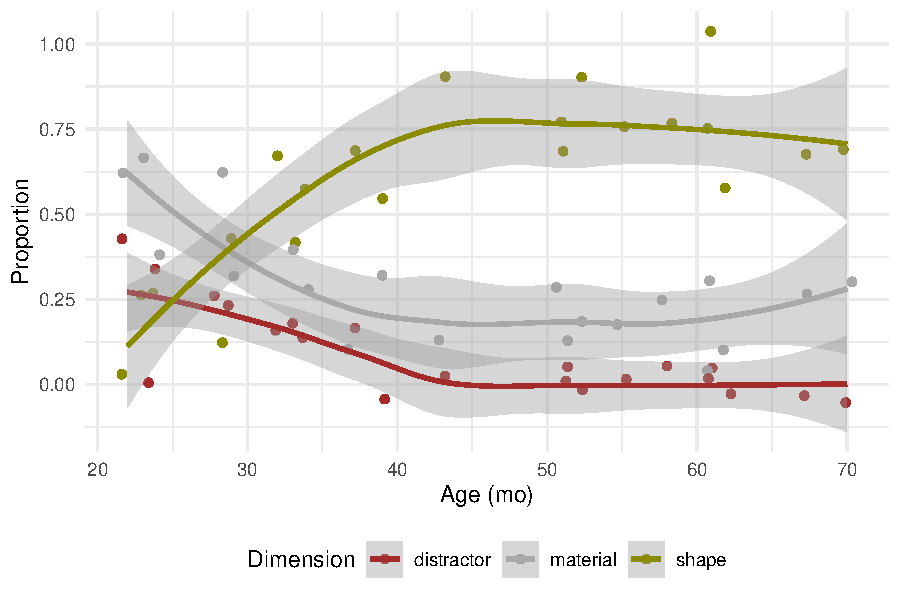
\includegraphics[width=1\linewidth]{figs/first_exp-1} \caption[Effect size plotted by average participant age]{Effect size plotted by average participant age. Points indicate individual effect, and error bars show variance. Points are colored based on language, and model fits for Indo-European and non-Indo-European languages are shown in black.}\label{fig:first_exp}
\end{figure}
\end{CodeChunk}

\hypertarget{experiment-2}{%
\subsection{Experiment 2}\label{experiment-2}}

\hypertarget{participants-1}{%
\subsubsection{Participants}\label{participants-1}}

31 (target n= 96, 24 per each age group from 2-5 years old) participants
(mean age = , sd, n per age group) were recruited from a local nursery
school in the US. demographic characteristics\ldots.

\hypertarget{stimuli-1}{%
\subsubsection{Stimuli}\label{stimuli-1}}

Same stimuli as above, but for the function test object, it is modified
in a way that doesn't change the shape at all, but allows for the
function (an object that is wrapped all over and a similar one that can
clearly open).

\hypertarget{procedure-1}{%
\subsubsection{Procedure:}\label{procedure-1}}

A within subject manipulation with two conditions: material or function.
The material condition is identical to the first experiment. In the
function condition, the experimenter introduce the exemplar object
``this is a dax'', gives the child 15 seconds seconds to play with it,
provides functional information `` the dax grapes toys'', gives another
15 seconds to play with it, and puts the toy away but within view,
before introducing the test objects and asks for a response.

\hypertarget{preliminary-results}{%
\subsubsection{Preliminary results}\label{preliminary-results}}

Similar to what is conveyed in Figure \ref{fig:jitter_function}, a
generalized random effects logistic model showed an overall tendency to
choose by shape regardless of condition 0.81 (\(p=\) .693) and a
positive trend with age 0.01 (\(p=\) .742) with a decline in shape bias
in the material condition -2.65 (\(p=\) .338). Little variability
between participants is displayed but a huge variability between stimuli
objects (\(sd=\) 1.35). Confidence intervals show uncertainty however
(data collection is still ongoing).

\begin{CodeChunk}
\begin{figure*}[tb]
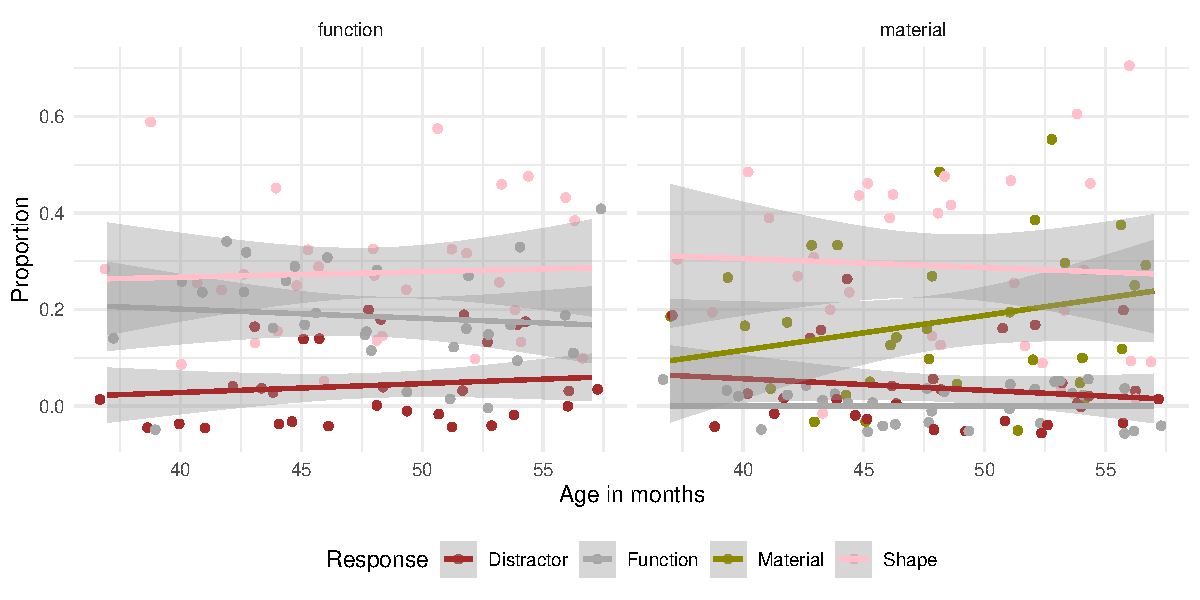
\includegraphics[width=1\linewidth]{figs/jitter_function-1} \caption[Effect size plotted by average participant age]{Effect size plotted by average participant age. Points indicate individual effect, and error bars show variance. Points are colored based on language, and model fits for Indo-European and non-Indo-European languages are shown in black.}\label{fig:jitter_function}
\end{figure*}
\end{CodeChunk}

\hypertarget{discussion}{%
\section{Discussion}\label{discussion}}

The word extension and category organization literature is highly
heterogeneous. Studies in this domain lack an integrative and
commensurable design, which hinders our ability to draw consistent
conclusions. To achieve a more accurate measurement of category
organization and concept learning, we need a reliable and valid wide
range set of stimuli objects, consistent task formats and test designs,
as well as multi-site cross-cultural experiments unified across
laboratories to maximally account for the variability. Our evaluation of
the word extension literature reveals that making procedural decisions,
which we think are likely a primary source of unexplained variability,
is unattianable without running a series of controlled experiments that
would allow us to systematically assess how different designs and
stimuli covary with response patterns. In our initial results, we see a
strong tendency to generalize by shape, even in conditions designed to
make function salient. This suggests that, even with a potential
saliency effect, where the trials highlighted functional information, it
failed to override the preference for shape-based choices. In additon,
many children explored whether their chosen test object could perform
the intended function after selecting it based on shape. This behavior
implies that the shape-based selection might not reflect a disregard for
functional information but rather a hypothesis that objects sharing
shape might also share functionality.

What does it mean to talk about validity and reliability in a task like
the word extension one? What is the construct we are talking about here.
It is a measure at the group level rather than at the individual level
\textgreater\textgreater{} this kid had this level of shape bias.
\textgreater\textgreater{} is it an issue of the signal is not even
there, or is it a matter of the level/degree of the signal when it comes
to cross-cultural work. (Madole, K. L., \& Oakes, L. M. (1999)):
Although the distinction between perceptual and conceptual categories
makes a certain intuitive sense, it may only confuse our attempts to
understand psychological reality. Establishing a reliable metric for
this distinction is extremely difficult and attempts to operationalize
the terms perceptual and conceptual are invariably highly ambiguous and
task-specific. How the perceptual vs conceptual debate maps into the
cross cultural differences debate ? As we mentioned in the introduction,
procedural variation observed in the literature have followed
theoretical debates and in fact reinforced by them. Thus, evaluating the
theories given the state of evidence is not feasbile and it will endup
crashing with this heterogeneity and with the broader question on the
type of knowledge being highlighted by each one of the evidence.

\hypertarget{general-formatting-instructions}{%
\section{General Formatting
Instructions}\label{general-formatting-instructions}}

For general information about authoring in markdown, see
\textbf{\href{http://rmarkdown.rstudio.com/authoring_basics.html}{here}.}

The entire content of a paper (including figures, references, and
anything else) can be no longer than six pages in the
\textbf{initial submission}. In the \textbf{final submission}, the text
of the paper, including an author line, must fit on six pages. Up to one
additional page can be used for acknowledgements and references.

The text of the paper should be formatted in two columns with an overall
width of 7 inches (17.8 cm) and length of 9.25 inches (23.5 cm), with
0.25 inches between the columns. Leave two line spaces between the last
author listed and the text of the paper; the text of the paper (starting
with the abstract) should begin no less than 2.75 inches below the top
of the page. The left margin should be 0.75 inches and the top margin
should be 1 inch. \textbf{The right and bottom margins will depend on
whether you use U.S. letter or A4 paper, so you must be sure to
measure the width of the printed text.} Use 10\textasciitilde point
Times Roman with 12\textasciitilde point vertical spacing, unless
otherwise specified.

The title should be in 14\textasciitilde point bold font, centered. The
title should be formatted with initial caps (the first letter of content
words capitalized and the rest lower case). In the initial submission,
the phrase ``Anonymous CogSci submission'\,' should appear below the
title, centered, in 11\textasciitilde point bold font. In the final
submission, each author's name should appear on a separate line,
11\textasciitilde point bold, and centered, with the author's email
address in parentheses. Under each author's name list the author's
affiliation and postal address in ordinary 10\textasciitilde point type.

Indent the first line of each paragraph by 1/8\textasciitilde inch
(except for the first paragraph of a new section). Do not add extra
vertical space between paragraphs.

\hypertarget{first-level-headings}{%
\section{First-Level Headings}\label{first-level-headings}}

First level headings should be in 12 point , initial caps, bold and
centered. Leave one line space above the heading and
1/4\textasciitilde line space below the heading.

\hypertarget{second-level-headings}{%
\subsection{Second-Level Headings}\label{second-level-headings}}

Second level headings should be 11 point , initial caps, bold, and flush
left. Leave one line space above the heading and 1/4\textasciitilde{}
line space below the heading.

\hypertarget{third-level-headings}{%
\subsubsection{Third-Level Headings}\label{third-level-headings}}

Third-level headings should be 10 point , initial caps, bold, and flush
left. Leave one line space above the heading, but no space after the
heading.

\hypertarget{formalities-footnotes-and-floats}{%
\section{Formalities, Footnotes, and
Floats}\label{formalities-footnotes-and-floats}}

Use standard APA citation format. Citations within the text should
include the author's last name and year. If the authors' names are
included in the sentence, place only the year in parentheses, as in
(1972), but otherwise place the entire reference in parentheses with the
authors and year separated by a comma (Newell \& Simon, 1972). List
multiple references alphabetically and separate them by semicolons
(Chalnick \& Billman, 1988; Newell \& Simon, 1972). Use the et.
al.~construction only after listing all the authors to a publication in
an earlier reference and for citations with four or more authors.

For more information on citations in RMarkdown, see
\textbf{\href{http://rmarkdown.rstudio.com/authoring_bibliographies_and_citations.html\#citations}{here}.}

\hypertarget{footnotes}{%
\subsection{Footnotes}\label{footnotes}}

Indicate footnotes with a number\footnote{Sample of the first
footnote.} in the text. Place the footnotes in 9 point type at the
bottom of the page on which they appear. Precede the footnote with a
horizontal rule.\footnote{Sample of the second footnote.} You can also
use markdown formatting to include footnotes using this syntax
\footnote{Sample of a markdown footnote.}.

\hypertarget{figures}{%
\subsection{Figures}\label{figures}}

All artwork must be very dark for purposes of reproduction and should
not be hand drawn. Number figures sequentially, placing the figure
number and caption, in 10 point, after the figure with one line space
above the caption and one line space below it. If necessary, leave extra
white space at the bottom of the page to avoid splitting the figure and
figure caption. You may float figures to the top or bottom of a column,
or set wide figures across both columns.

\hypertarget{two-column-images}{%
\subsection{Two-column images}\label{two-column-images}}

You can read local images using png package for example and plot it like
a regular plot using grid.raster from the grid package. With this method
you have full control of the size of your image. \textbf{Note: Image
must be in .png file format for the readPNG function to work.}

You might want to display a wide figure across both columns. To do this,
you change the \texttt{fig.env} chunk option to \texttt{figure*}. To
align the image in the center of the page, set \texttt{fig.align} option
to \texttt{center}. To format the width of your caption text, you set
the \texttt{num.cols.cap} option to \texttt{2}.

\begin{CodeChunk}
\begin{figure*}[h]

{\centering 
\includegraphics{figs/2-col-image-1} 

}

\caption[This image spans both columns]{This image spans both columns. And the caption text is limited to 0.8 of the width of the document.}\label{fig:2-col-image}
\end{figure*}
\end{CodeChunk}

\hypertarget{one-column-images}{%
\subsection{One-column images}\label{one-column-images}}

Single column is the default option, but if you want set it explicitly,
set \texttt{fig.env} to \texttt{figure}. Notice that the
\texttt{num.cols} option for the caption width is set to \texttt{1}.

\begin{CodeChunk}
\begin{figure}[H]

{\centering 
\includegraphics{figs/image-1} 

}

\caption[One column image]{One column image.}\label{fig:image}
\end{figure}
\end{CodeChunk}

\hypertarget{r-plots}{%
\subsection{R Plots}\label{r-plots}}

You can use R chunks directly to plot graphs. And you can use latex
floats in the fig.pos chunk option to have more control over the
location of your plot on the page. For more information on latex
placement specifiers see
\textbf{\href{https://en.wikibooks.org/wiki/LaTeX/Floats,_Figures_and_Captions}{here}}

\begin{CodeChunk}
\begin{figure}[H]

{\centering 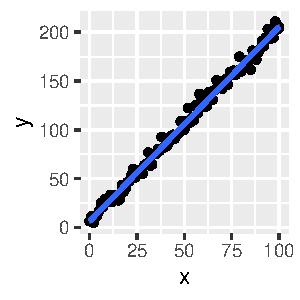
\includegraphics{figs/plot-1} 

}

\caption[R plot]{R plot}\label{fig:plot}
\end{figure}
\end{CodeChunk}

\hypertarget{tables}{%
\subsection{Tables}\label{tables}}

Number tables consecutively; place the table number and title (in 10
point) above the table with one line space above the caption and one
line space below it, as in Table 1. You may float tables to the top or
bottom of a column, set wide tables across both columns.

You can use the xtable function in the xtable package.

\begin{table}[H]
\centering
\begin{tabular}{rrrrr}
  \hline
 & Estimate & Std. Error & t value & Pr($>$$|$t$|$) \\ 
  \hline
(Intercept) & 0.05 & 0.10 & 0.5 & 0.62 \\ 
  x & 2.01 & 0.10 & 20.1 & 0.00 \\ 
   \hline
\end{tabular}
\caption{This table prints across one column.} 
\end{table}

\hypertarget{acknowledgements}{%
\section{Acknowledgements}\label{acknowledgements}}

Place acknowledgments (including funding information) in a section at
the end of the paper.

\hypertarget{references}{%
\section{References}\label{references}}

\setlength{\parindent}{-0.1in} 
\setlength{\leftskip}{0.125in}

\noindent

\hypertarget{refs}{}
\begin{CSLReferences}{1}{0}
\leavevmode\vadjust pre{\hypertarget{ref-abdelrahim_frank_2024}{}}%
Abdelrahim, S., \& Frank, M. C. (2024, September). Examining the
robustness and generalizability of the shape bias: A meta-analysis.
PsyArXiv.
http://doi.org/\href{https://doi.org/10.31234/osf.io/3by54}{10.31234/osf.io/3by54}

\leavevmode\vadjust pre{\hypertarget{ref-Baldwin1992ClarifyingTR}{}}%
Baldwin, D. A. (1992). Clarifying the role of shape in children's
taxonomic assumption. \emph{Journal of Experimental Child Psychology},
\emph{54 3}, 392--416. Retrieved from
\url{https://api.semanticscholar.org/CorpusID:29725812}

\leavevmode\vadjust pre{\hypertarget{ref-ChalnickBillman1988a}{}}%
Chalnick, A., \& Billman, D. (1988). Unsupervised learning of
correlational structure. In \emph{Proceedings of the tenth annual
conference of the cognitive science society} (pp. 510--516). Hillsdale,
NJ: Lawrence Erlbaum Associates.

\leavevmode\vadjust pre{\hypertarget{ref-CLARK197365}{}}%
CLARK, E. V. (1973). WHAT's IN a WORD? ON THE CHILD's ACQUISITION OF
SEMANTICS IN HIS FIRST LANGUAGE11This research was supported in part by
NSF grant GS-1880 to the language universals project, stanford
university, and in part by NSF grant GS-30040 to the author. In T. E.
Moore (Ed.), \emph{Cognitive development and acquisition of language}
(pp. 65--110). San Diego: Academic Press.
http://doi.org/\url{https://doi.org/10.1016/B978-0-12-505850-6.50009-8}

\leavevmode\vadjust pre{\hypertarget{ref-colunga2000learning}{}}%
Colunga, E., \& Smith, L. B. (2000). Learning to learn words: A
cross-linguistic study of the shape and material biases. In
\emph{Proceedings of the 24th annual boston university conference on
language development} (Vol. 1, pp. 197--207).

\leavevmode\vadjust pre{\hypertarget{ref-gathercole_1997}{}}%
Gathercole, V. C. M., \& Min, H. (1997). Word meaning biases or
language-specific effects? {Evidence} from {English}, {Spanish} and
{Korean}. \emph{First Language}, \emph{17}(51), 031--56.
http://doi.org/\href{https://doi.org/10.1177/014272379701705102}{10.1177/014272379701705102}

\leavevmode\vadjust pre{\hypertarget{ref-gershkoff2004shape}{}}%
Gershkoff-Stowe, L., \& Smith, L. B. (2004). Shape and the first hundred
nouns. \emph{Child Development}, \emph{75}(4), 1098--1114.

\leavevmode\vadjust pre{\hypertarget{ref-graham_2010}{}}%
Graham, S. A., \& Diesendruck, G. (2010). Fifteen-month-old infants
attend to shape over other perceptual properties in an induction task.
\emph{Cognitive Development}, \emph{25}(2), 111--123.
http://doi.org/\href{https://doi.org/10.1016/j.cogdev.2009.06.002}{10.1016/j.cogdev.2009.06.002}

\leavevmode\vadjust pre{\hypertarget{ref-Graham1999InfantsRO}{}}%
Graham, S. A., \& Poulin-Dubois, D. (1999). Infants' reliance on shape
to generalize novel labels to animate and inanimate objects.
\emph{Journal of Child Language}, \emph{26}, 295--320. Retrieved from
\url{https://api.semanticscholar.org/CorpusID:43424185}

\leavevmode\vadjust pre{\hypertarget{ref-imai1997}{}}%
Imai, M., \& Gentner, D. (1997). A cross-linguistic study of early word
meaning: Universal ontology and linguistic influence. \emph{Cognition},
\emph{62}(2), 169--200.

\leavevmode\vadjust pre{\hypertarget{ref-imai_childrens_1994}{}}%
Imai, M., Gentner, D., \& Uchida, N. (1994). Children's theories of word
meaning: {The} role of shape similarity in early acquisition.
\emph{Cognitive Development}, \emph{9}(1), 45--75.
http://doi.org/\href{https://doi.org/10.1016/0885-2014(94)90019-1}{10.1016/0885-2014(94)90019-1}

\leavevmode\vadjust pre{\hypertarget{ref-jara2022}{}}%
Jara-Ettinger, J., Levy, R., Sakel, J., Huanca, T., \& Gibson, E.
(2022). The origins of the shape bias: Evidence from the tsimane'.
\emph{Journal of Experimental Psychology: General}.

\leavevmode\vadjust pre{\hypertarget{ref-Jones2003}{}}%
Jones, S. S. (2003). Late talkers show no shape bias in a novel name
extension task. \emph{Developmental Science}, \emph{6}(5), 477--483.
http://doi.org/\url{https://doi.org/10.1111/1467-7687.00304}

\leavevmode\vadjust pre{\hypertarget{ref-JONES_SMITH_2005}{}}%
JONES, S. S., \& SMITH, L. B. (2005). Object name learning and object
perception: A deficit in late talkers. \emph{Journal of Child Language},
\emph{32}(1), 223--240.
http://doi.org/\href{https://doi.org/10.1017/S0305000904006646}{10.1017/S0305000904006646}

\leavevmode\vadjust pre{\hypertarget{ref-LANDAU1988299}{}}%
Landau, B., Smith, L. B., \& Jones, S. S. (1988). The importance of
shape in early lexical learning. \emph{Cognitive Development},
\emph{3}(3), 299--321.
http://doi.org/\url{https://doi.org/10.1016/0885-2014(88)90014-7}

\leavevmode\vadjust pre{\hypertarget{ref-Nelson1974ConceptWA}{}}%
Nelson, K. (1974). Concept, word, and sentence: Interrelations in
acquisition and development. \emph{Psychological Review}, \emph{81},
267--285. Retrieved from
\url{https://api.semanticscholar.org/CorpusID:143965074}

\leavevmode\vadjust pre{\hypertarget{ref-NewellSimon1972a}{}}%
Newell, A., \& Simon, H. A. (1972). \emph{Human problem solving}.
Englewood Cliffs, NJ: Prentice-Hall.

\leavevmode\vadjust pre{\hypertarget{ref-perry2010learn}{}}%
Perry, L. K., Samuelson, L. K., Malloy, L. M., \& Schiffer, R. N.
(2010). Learn locally, think globally: Exemplar variability supports
higher-order generalization and word learning. \emph{Psychological
Science}, \emph{21}(12), 1894--1902.

\leavevmode\vadjust pre{\hypertarget{ref-samuelson_statistical_2002}{}}%
Samuelson, Larissa K. (2002). Statistical regularities in vocabulary
guide language acquisition in connectionist models and 15-20-month-olds.
\emph{Developmental Psychology}, \emph{38}(6), 1016--1037.
http://doi.org/\href{https://doi.org/10.1037/0012-1649.38.6.1016}{10.1037/0012-1649.38.6.1016}

\leavevmode\vadjust pre{\hypertarget{ref-samuelson2008rigid}{}}%
Samuelson, Larissa K., Horst, J. S., Schutte, A. R., \& Dobbertin, B. N.
(2008). Rigid thinking about deformables: Do children sometimes
overgeneralize the shape bias? \emph{Journal of Child Language},
\emph{35}(3), 559--589.

\leavevmode\vadjust pre{\hypertarget{ref-samuelson1999}{}}%
Samuelson, Larissa K., \& Smith, L. B. (1999). Early noun vocabularies:
Do ontology, category structure and syntax correspond? \emph{Cognition},
\emph{73}(1), 1--33.

\leavevmode\vadjust pre{\hypertarget{ref-samuelson2000children}{}}%
Samuelson, Larissa K., \& Smith, L. B. (2000). Children's attention to
rigid and deformable shape in naming and non-naming tasks. \emph{Child
Development}, \emph{71}(6), 1555--1570.

\leavevmode\vadjust pre{\hypertarget{ref-smithcolunga2010}{}}%
Smith, L. B., Colunga, E., \& Yoshida, H. (2010). Knowledge as process:
Contextually cued attention and early word learning. \emph{Cognitive
Science}, \emph{34}(7), 1287--1314.
http://doi.org/\url{https://doi.org/10.1111/j.1551-6709.2010.01130.x}

\leavevmode\vadjust pre{\hypertarget{ref-smith_object_2002}{}}%
Smith, L. B., Jones, S. S., Landau, B., Gershkoff-Stowe, L., \&
Samuelson, L. (2002). Object name learning provides on-the-job training
for attention. \emph{Psychological Science}, \emph{13}(1), 13--19.
http://doi.org/\href{https://doi.org/10.1111/1467-9280.00403}{10.1111/1467-9280.00403}

\leavevmode\vadjust pre{\hypertarget{ref-soja1991ontological}{}}%
Soja, Nancy N., Carey, S., \& Spelke, E. S. (1991). Ontological
categories guide young children's inductions of word meaning: Object
terms and substance terms. \emph{Cognition}, \emph{38}(2), 179--211.

\leavevmode\vadjust pre{\hypertarget{ref-soja_perception_1992}{}}%
Soja, Nancy N., Carey, S., \& Spelke, E. S. (1992). Perception,
ontology, and word meaning. \emph{Cognition}, \emph{45}(1), 101--107.
http://doi.org/\href{https://doi.org/10.1016/0010-0277(92)90025-D}{10.1016/0010-0277(92)90025-D}

\leavevmode\vadjust pre{\hypertarget{ref-subrahmanyam_2006}{}}%
Subrahmanyam, K., \& Chen, H.-H. N. (2006). A crosslinguistic study of
children's noun learning: {The} case of object and substance words.
\emph{First Language}, \emph{26}(2), 141--160.
http://doi.org/\href{https://doi.org/10.1177/0142723706060744}{10.1177/0142723706060744}

\leavevmode\vadjust pre{\hypertarget{ref-yoshida2003known}{}}%
Yoshida, H., \& Smith, L. B. (2003a). Known and novel noun extensions:
Attention at two levels of abstraction. \emph{Child Development},
\emph{74}(2), 564--577.

\leavevmode\vadjust pre{\hypertarget{ref-yoshida2003}{}}%
Yoshida, H., \& Smith, L. B. (2003b). Shifting ontological boundaries:
How japanese-and english-speaking children generalize names for animals
and artifacts. \emph{Developmental Science}, \emph{6}(1), 1--17.

\end{CSLReferences}

\bibliographystyle{apacite}


\end{document}
